We define the following sets of monomorphisms from $X$ to $G$ to facilitate the discussion of the termination criterion. They are almost identical to the ones defined in Notation~\ref{subgraph_counting:notation:mono_sets}. The only difference is that the first parameter is a ruler-graph $\mathcal{X}=(X,f)$ defined in Definition~\ref{antipattern:def:ruler_graph} instead of the underlying graph $X$.
\begin{notation}
    \label{antipattern:notation:mono_sets}
     \ \newline
\noindent
\begin{minipage}{0.69\textwidth}
\vspace{2mm}
\noindent 
  Let \( \mathcal{X}\) be a ruler-graph with underlying graph $X$. The disjoint union of two sets \( S \) and \( S' \) will be denoted by \( S \uplus S' \). Let \( X, A, B, G \) be graphs, and let \( \alpha \colon A \to G \) and \( \beta \colon B \to G \) be morphisms as illustrated on the right. We define the following sets of monomorphisms from $X$ in $G$ based on their interaction with $\alpha$ and $\beta$:    
\end{minipage}% 
\begin{minipage}{0.30\textwidth}
    \hfill
        \resizebox{0.9\textwidth}{!}{
        % \begin{tikzpicture}
        %     \node (B) at (2,0) {$A$}; 
        %     \node (C) at (0,2) {$B$}; 
        %     \node (D) at (0,0) {$G$}; 
        %     \draw [>->] (B) to node [below,label,pos=0.45] {$\alpha$} (D); 
        %     \draw [>->] (C) to node [left,label,pos=0.45] {$\beta$} (D);
        % \end{tikzpicture}
            \begin{tikzpicture}
            \node (X) at (-1.5,-1) {$X$};
            \node (B) at (2,0) {$A$}; 
            \node (C) at (0,2) {$B$}; 
            \node (D) at (0,0) {$G$}; 
            \draw [>->] (B) to node [above,label,pos=0.45] {$\alpha$} (D); 
            \draw [>->] (C) to node [right,label,pos=0.45] {$\beta$} (D);
            \draw [>->,dashed] (X) to node [above,label,pos=0.45] {$\iota$} (D);
            \draw [>->,dashed] (X) to node [below,label,pos=0.45] {$\zeta$} (B);
            \draw [>->,dashed] (X) to node [above,label,pos=0.45] {$\eta$} (C);
        \end{tikzpicture}
        }
\end{minipage} 
    \begin{align*}
        \operatorname{Mono}(\mathcal{X},G) &= \operatorname{Mono}(X,G), 
        \\
        \operatorname{Mono}(\mathcal{X},G,\alpha) &= \left\{ \iota \colon X \rightarrowtail G 
        \;\middle|\; 
        \exists \zeta \colon X \rightarrowtail A.\, \iota = \zeta \star \alpha \right\}, 
        \\
        \operatorname{Mono}(\mathcal{X},G,\lnot \alpha) &= \left\{ \iota \colon X \rightarrowtail G 
        \;\middle|\; 
        \nexists \zeta \colon X \rightarrowtail A.\, \iota = \zeta \star \alpha \right\}, 
        \\
        \operatorname{Mono}(\mathcal{X},G,\lnot \alpha, \beta) &= \left\{ 
            \iota \colon X \rightarrowtail G \;\middle|\; 
                \begin{aligned}  
                    &(\nexists \zeta \colon X \rightarrowtail A.\, \iota = \zeta \star \alpha) \\ 
                    &\land (\exists \eta \colon X \rightarrowtail B.\, \iota = \eta \star \beta)
                \end{aligned}
        \right\},
        \\
        \operatorname{Mono}(\mathcal{X},G,\lnot \alpha, \lnot \beta) &= \left\{ 
            \iota \colon X \rightarrowtail G \;\middle|\; 
                \begin{aligned}
                    &(\nexists \zeta \colon X \rightarrowtail A.\, \iota = \zeta \star \alpha) \\
                    &\land (\nexists \eta \colon X \rightarrowtail B.\, \iota = \eta \star \beta)
                \end{aligned}
        \right\}.
    \end{align*}
    For a set $\operatorname{Mono}(\mathcal{X},\dots)$, we define $\operatorname{Mono}(\mathcal{X},\dots)_{\operatorname{NF}}$ as the subset of \( X \)-occurrences whose images are not included in any occurrence of its forbidden context if exists, and  $\operatorname{Mono}(\mathcal{X},\dots)_{\operatorname{F}}$ as the subset of \( X \)-occurrences whose images are included in some occurrences of its forbidden context if exists. 
\end{notation}
\noindent
\begin{minipage}{0.7\textwidth}\setlength{\parindent}{1em}
    Let $\mathcal{X}$ be a ruler-graph with underlying graph $X$ and \( \rho = (L \overset{l}{\leftarrowtail} K \overset{r}{\rightarrowtail} R) \) be a rule. 
    Consider the DPO diagram illustrated on the right. 
\end{minipage}%
\begin{minipage}{0.29\textwidth}
    \hfill
    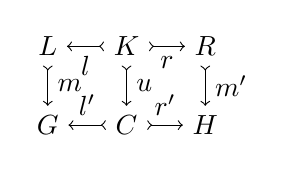
\begin{tikzpicture}
        % [node distance=15mm]
        \node (I) {$K$};
        \node (L) [left of=I] {$L$};
        \node (R) [right of=I] {$R$};
        \node (G) [below of=L] {$G$};
        \node (C) [below of=I] {$C$};
        \node (H) [below of=R] {$H$}; 
        \draw [>->] (I) to  node [midway,below] {$l$} (L);
        \draw [>->] (I) to  node [midway,below] {$r$} (R);
        \draw [>->] (L) to node [midway,right] {$m$} (G);
        \draw [>->] (I) to  node [midway,right] {$u$} (C); 
        \draw [>->] (R) to  node [midway,right] {$m'$} (H);
        \draw [>->] (C) to node [midway,above] {$l'$} (G);
        \draw [>->] (C) to node [midway,above] {$r'$} (H);
        % \node [at=($(I)!.5!(G)$)] {\normalfont PO};
        % \node [at=($(I)!.5!(H)$)] {\normalfont PO};
      \end{tikzpicture}
\end{minipage} 

\vspace{1mm}
% The following decompositions hold:
% \begin{flalign*}
%     \operatorname{Mono}(\mathcal{X},G)_{\operatorname{NF}} &= 
%     \operatorname{Mono}(\mathcal{X},G,m)_{\operatorname{NF}}
%     \uplus
%     \operatorname{Mono}(\mathcal{X},G,\lnot m, l')_{\operatorname{NF}} 
%     \uplus
%     \operatorname{Mono}(\mathcal{X},G,\lnot m, \lnot l')_{\operatorname{NF}}
%     \\
%     \operatorname{Mono}(\mathcal{X},H)_{\operatorname{NF}} &= 
%     \operatorname{Mono}(\mathcal{X},H,m')_{\operatorname{NF}}
%     \uplus
%     \operatorname{Mono}(\mathcal{X},H,\lnot m', r')_{\operatorname{NF}}
%     \uplus
%     \operatorname{Mono}(\mathcal{X},H,\lnot m', \lnot r')_{\operatorname{NF}}
% \end{flalign*}

The set $\operatorname{Mono}(\mathcal{X},G)_{\operatorname{NF}}$ can be partitioned into three disjoint sets:
$$
    \operatorname{Mono}(\mathcal{X},G,m)_{\operatorname{NF}}
    \uplus
    \operatorname{Mono}(\mathcal{X},G,\lnot m, l')_{\operatorname{NF}} 
    \uplus
    \operatorname{Mono}(\mathcal{X},G,\lnot m, \lnot l')_{\operatorname{NF}}
$$
and $\operatorname{Mono}(\mathcal{X},H)_{\operatorname{NF}}$ can be partitioned into three disjoint sets:
$$
\operatorname{Mono}(\mathcal{X},H,m')_{\operatorname{NF}}
    \uplus
    \operatorname{Mono}(\mathcal{X},H,\lnot m', r')_{\operatorname{NF}}
    \uplus
    \operatorname{Mono}(\mathcal{X},H,\lnot m', \lnot r')_{\operatorname{NF}}
$$
Thus, we have 
\begin{flalign}
    &\card{\operatorname{Mono}(\mathcal{X},G)_{\operatorname{NF}}} - 
    \card{\operatorname{Mono}(\mathcal{X},H)_{\operatorname{NF}}} \nonumber
    \\=
    &(\card{\operatorname{Mono}(\mathcal{X},G,m)_{\operatorname{NF}}} 
        -  
    \card{\operatorname{Mono}(\mathcal{X},H,m')_{\operatorname{NF}}}) 
    +  \nonumber
    \\
    &(
        \card{\operatorname{Mono}(\mathcal{X},G,\lnot m, l')_{\operatorname{NF}}}
             - 
        \card{\operatorname{Mono}(\mathcal{X},H,\lnot m', r')_{\operatorname{NF}}}) +  \nonumber \\ 
    &(
        \card{\operatorname{Mono}(\mathcal{X},G,\lnot m, \lnot l')_{\operatorname{NF}}} 
            - 
        \card{\operatorname{Mono}(\mathcal{X},H,\lnot m', \lnot r')_{\operatorname{NF}}} \nonumber
    )
\end{flalign}
In the remainder of this section, we suppose that $\rho^{-1}$ is $F$-non-increasing if $\mathcal{X}= (X,f:X \rightarrowtail F)$ and, $\rho$ and $\rho^{-1}$ are $X$-non-increasing. To estimate $\card{\operatorname{Mono}(\mathcal{X},G)_{\operatorname{NF}}} - 
    \card{\operatorname{Mono}(\mathcal{X},H)_{\operatorname{NF}}}$, we establish the following lemmas.
% The following lemmas can be used to approximate $\card{\operatorname{Mono}(\mathcal{X},G)_{\operatorname{NF}}} - 
%     \card{\operatorname{Mono}(\mathcal{X},H)_{\operatorname{NF}}}$
\begin{lemma}
    \label{antipattern:lem:xglnotmlp_xhlnotmrp}
        Let $\mathcal{X}$ be a ruler-graph with underlying graph $X$ and \( \rho = (L \overset{l}{\leftarrowtail} K \overset{r}{\rightarrowtail} R) \) be a rule. 
        Suppose that $\rho^{-1}$ is $F$-non-increasing if $\mathcal{X} = (X,f:X \rightarrowtail F)$.
        We have 
    $$\card{\operatorname{Mono}(\mathcal{X},G,\lnot m, l')_{\operatorname{NF}}} \geq
        \card{\operatorname{Mono}(\mathcal{X},H,\lnot m', r')_{\operatorname{NF}}}$$
\end{lemma} 
See~\textsection~\ref{antipattern:proof:lem:xglnotmlp_xhlnotmrp} for the proof of this lemma.
\begin{lemma}
    \label{antipattern:lem:xglnotmlnotlp_xhlnotmrnotrp}
        Let $\mathcal{X}$ be a ruler-graph with underlying graph $X$ and let \( \rho = (L \overset{l}{\leftarrowtail} K \overset{r}{\rightarrowtail} R) \) be a rule. Suppose that $\rho$ and $\rho^{-1}$ are $X$-non-increasing. We have
    $$ 
        \card{\operatorname{Mono}(\mathcal{X},G,\lnot m, \lnot l')_{\operatorname{NF}}} \geq
        \card{\operatorname{Mono}(\mathcal{X},H,\lnot m', \lnot r')_{\operatorname{NF}}}
    $$
\end{lemma}
See~\textsection~\ref{antipattern:proof:lem:xglnotmlnotlp_xhlnotmrnotrp} for the proof of this lemma.
Under the assumptions of the above two lemmas, we can estimate the following inequality.
 \begin{flalign*}
     \card{\operatorname{Mono}(\mathcal{X},G)_{\operatorname{NF}}} - 
     \card{\operatorname{Mono}(\mathcal{X},H)_{\operatorname{NF}}} 
     \geq
     \card{\operatorname{Mono}(\mathcal{X},G,m)_{\operatorname{NF}}} - \card{\operatorname{Mono}(\mathcal{X},H,m')_{\operatorname{NF}}}
 \end{flalign*}

\begin{definition}
    \label{antipattern:def:gamma_l_rho_x}
    Let $\mathcal{X}$ be a ruler-graph with underlying graph $X$. 
    Let \( \rho = (L \overset{l}{\leftarrowtail} K \overset{r}{\rightarrowtail} R) \) be a rule.
    Define $\Gamma(\operatorname{Mono}(\mathcal{X},L)_{\operatorname{NF}})$ as the subset of $\operatorname{Mono}(\mathcal{X},L)_{\operatorname{NF}}$ consisting of $X$-occurrences whose images are not included in any occurrence of the forbidden context in $L$,
    but, in some rewriting step $G \Rightarrow_\rho^m H$, their images may possibly be included in some occurrence of the forbidden context in the host graph $G$.
    Formally,  $\Gamma(\operatorname{Mono}(\mathcal{X},L)_{\operatorname{NF}}) = \emptyset$ if $\mathcal{X} = (X)$, and if $\mathcal{X} = (X, f:X \rightarrowtail F)$, then a monomorphism $h_{XL}:X \rightarrowtail L$ is in $\Gamma(\operatorname{Mono}(\mathcal{X},L)_{\operatorname{NF}})$ iff the following hold:
    \begin{itemize}
        \item there does not exist $h_{FL}:F \rightarrowtail L$ such that $f \star h_{FL} = h_{XL}$,
         \item there exists a graph $C$ and a monomorphism $h_{KC}:K \overset{u}{\rightarrowtail} C$ such that, let $L \overset{m}{\rightarrowtail} G \overset{l'}{\leftarrowtail} C$ be the pushout of the span $L \overset{l}{\leftarrowtail} K \overset{u}{\rightarrowtail} C$, as illustrated in Figure~\ref{fig:antipattern:def:gamma_l_rho_x},
         there exist a monomorphism $h_{FG} : F \rightarrowtail G$ such that 
        %  $h_{XL} \star h_{LG} = h_{XF} \star h_{FG}$
         $h_{XL} \star m = h_{XF} \star h_{FG}$. 
      \begin{center}
        \resizebox{0.3\textwidth}{!}{
            \begin{tikzpicture}
                    \node (k) at (0,1) {K};
                    \node (l) at (-2,1) {L};
                    \node (c) at (0,-1) {C};
                    \node (g) at (-2,-1) {G};
                    \node (x) at (-4,-2) {X};
                    \node (f) at (-2,-2) {F};
                    \draw[<-<]  (l) -- (k) node [midway,below] {$l$};
                    \draw[>->] (c) -- (g) node [midway, above] {$l'$};
                    \draw[>->] (l) -- (g) node[midway, right] {$m$};
                    \draw[>->] (k) -- (c) node[midway, left] {$u$};
                    \draw[>->] (x) -- (l) node[midway, left] {$h_{XL}$};
                    \draw[>->] (x) -- (f) node[midway, above] {$f$};
                    \draw[>->] (f) -- (g) node[midway, right] {$h_{FG}$};
                    \node () [at=($(l)!0.5!(c)$)] {$PO$};
                \end{tikzpicture}
         }
        %  \caption{}
        %  \label{fig:antipattern:def:gamma_l_rho_x}
        %     \end{figure}
        \end{center}
    \end{itemize}
    Furthermore, we define $\Lambda(\mathcal{X},\rho) \overset{\operatorname{def}}{=} (\card{\operatorname{Mono}(\mathcal{X},L)_{\operatorname{NF}}} - 
    \card{\Gamma(\operatorname{Mono}(\mathcal{X},L)_{\operatorname{NF}})}) -
   \card{\operatorname{Mono}(\mathcal{X},R)_{\operatorname{NF}}}$ to improve the readability of the following discussion.
%    \trackedtext{Intuitively, $\Lambda(\mathcal{X},\rho)$ is the number of $X$-occurrences in $L$ ...}
\end{definition}
Note that in category \textbf{Graph}, the pushout of two arrows always exists~\cite[p.188]{corradini1997algebraic}. Which justifies the existence of the pushout square in the second condition of the above definition.
Furthermore, since $X$ and the forbidden context (if exists) are finite graphs, $\Lambda(\mathcal{X},\rho)$ can be precisely computed. Consequently, it provides a lower bound for the change in the number of $X$-occurrences in a rewriting step using $\rho$, as shown in the following lemma whose proof is given in~\textsection~\ref{antipattern:proof:lem:xgm_xhmp_xl_xr}.

% \begin{lemma}
%     \label{lem:decomp_w_u}
%     \ \newline
%     \noindent
%     \begin{minipage}{0.7\textwidth}
%         Let $X$ be a ruler-graph. For a pushout square as shown on the right, we have 
%         % $\card{\operatorname{Mono}(X, B)} = \card{\operatorname{Mono}(X, D, \beta')}$ and $\card{\operatorname{Mono}(X, C, \lnot \beta)} = \card{\operatorname{Mono}(X, D, \lnot \beta', \alpha')}$.
%         \begin{flalign*}
%             \card{\operatorname{Mono}(X, B)} &= \card{\operatorname{Mono}(X, D, \beta')}
%             \\
%             \card{\operatorname{Mono}(X, C, \lnot \beta)} &= \card{\operatorname{Mono}(X, D, \lnot \beta', \alpha')}
%         \end{flalign*}
%     \end{minipage}
%     \hfill
%     \begin{minipage}{0.3\textwidth}
%         \hfill
%         \begin{tikzpicture}
%             \node (A) {$A$};
%             \node [below of=A] (B) {$B$}; 
%             \node [left of=A] (C) {$C$}; 
%             \node [left of=B] (D) {$D$}; 
%             \begin{scope}[nodes=rectangle]          
%             \draw [>->] (A) to node [right,label,pos=0.5] {$\alpha$} (B);
%             \draw [>->] (A) to node [above,label,pos=0.5] {$\beta$} (C);
%             \draw [>->] (B) to node [below,label,pos=0.45] {$\beta'$} (D); 
%             \draw [>->] (C) to node [left,label,pos=0.45] {$\alpha'$} (D);
%             \end{scope}
%         \end{tikzpicture}
%     \end{minipage} 
% \end{lemma}
% \begin{proof}
%     See the Appendix,~\autoref{proof:dcomp_w_u}.
%  \end{proof}
% \begin{lemma}
%     \label{lem:xgm_xhmp_xl_xr}
%     % If the number of $X$-occurrences that are not  included in any occurrences of forbidden context $F \in F_x$ in a $\rho$-rewriting step is predictable, then
%     $
%         \card{\operatorname{Mono}(\mathcal{X},G,m)_{\operatorname{NF}}} - 
%         \card{\operatorname{Mono}(\mathcal{X},H,m')_{\operatorname{NF}}} 
%         \geq 
%         \card{\operatorname{Mono}(X,L)} -
%         \card{\operatorname{Mono}(X,R)}
%     $
% \end{lemma}
% \begin{proof}
%     See the Appendix, \textsection~\ref{proof:lem:xgm_xhmp_xl_xr}.
%  \end{proof}

\begin{lemma}
    \label{antipattern:lem:xgm_xhmp_xl_xr}
     Let $\mathcal{X} = (X, f:X \rightarrowtail F)$ be a ruler-graph and \( \rho = (L \overset{l}{\leftarrowtail} K \overset{r}{\rightarrowtail} R) \) be a rule. 
   We have
    \begin{flalign*}
        &\card{\operatorname{Mono}(\mathcal{X},G,m)_{\operatorname{NF}}} - 
        \card{\operatorname{Mono}(\mathcal{X},H,m')_{\operatorname{NF}}} 
        \geq
        \Lambda(\mathcal{X},\rho)
    \end{flalign*}
\end{lemma}
 Thus, by the unnumbered equation preceding Definition~\ref{antipattern:def:gamma_l_rho_x},  we can conclude that
 \begin{flalign}
         \card{\operatorname{Mono}(\mathcal{X},G)_{\operatorname{NF}}} - 
     \card{\operatorname{Mono}(\mathcal{X},H)_{\operatorname{NF}}} 
     \geq 
    \Lambda(\mathcal{X},\rho)
     \label{eq:mono_x_g_nf_mono_x_h_nf_geq}
 \end{flalign}
Consequently, we have  
\begin{flalign*}
    &w_{s_\mathbb{X}}(G) - w_{s_\mathbb{X}}(H)
    \\
   \overset{\operatorname{def}}{=}&\sum_{\mathcal{X} \in \mathbb{X}}^{}s_\mathbb{X}(X) * m_X(G) - \sum_{\mathcal{X} \in \mathbb{X}}^{}s_\mathbb{X}(X) * m_X(H)
   \\
   \overset{\operatorname{def}}{=}&\sum_{\mathcal{X} \in \mathbb{X}}^{}s_\mathbb{X}(X) * |\operatorname{Mono}(\mathcal{X},G)_{\operatorname{NF}}| - \sum_{\mathcal{X} \in \mathbb{X}}^{}s_\mathbb{X}(X) * |\operatorname{Mono}(\mathcal{X},H)_{\operatorname{NF}}|
   \\
   =&\sum_{\mathcal{X} \in \mathbb{X}}^{}s_\mathbb{X}(X) * \left( \card{\operatorname{Mono}(\mathcal{X},G)_{\operatorname{NF}}} - 
   \card{\operatorname{Mono}(\mathcal{X},H)_{\operatorname{NF}}} \right)
   \\
   \geq&\sum_{\mathcal{X} \in \mathbb{X}}^{}s_\mathbb{X}(X) * \Lambda(\mathcal{X},\rho)
   & \text{by Equation~\eqref{eq:mono_x_g_nf_mono_x_h_nf_geq}}
%    \\
%    =&\sum_{\mathcal{X} \in \mathbb{X}}^{}s_\mathbb{X}(X) * \card{\operatorname{Mono}(X,G)} -  
%    \sum_{\mathcal{X} \in \mathbb{X}}^{}s_\mathbb{X}(X) *  \card{\operatorname{Mono}(X,H)}  
%     \\
%     \overset{\operatorname{def}}{=}&\sum_{\mathcal{X} \in \mathbb{X}}^{}s_\mathbb{X}(X) * m_X(L) - \sum_{\mathcal{X} \in \mathbb{X}}^{}s_\mathbb{X}(X) * m_X(R)
%     \\
%     \overset{\operatorname{def}}{=}& w_{s_\mathbb{X}}(L) - w_{s_\mathbb{X}}(R)
\end{flalign*} 
Which proves the following key lemma of this section.
\begin{lemma}[Decreasing step]
    \label{antipattern:lem:w_g_geq_w_h_leq}
    Let $\rho = (L \overset{l}{\leftarrowtail} K \overset{r}{\rightarrowtail} R)$ be an injective DPO rewriting rule,
    \( \mathbb{X} \) a set of ruler-graphs,
    \( s_{\mathbb{X}} \colon \mathbb{X} \to \mathbb{N} \) a weight function,
    and \( G \Rightarrow_{\rho,\mathfrak{M}} H \) a rewriting step. 
    Suppose that for every \( \mathcal{X} \in \mathbb{X} \) with underlying graph $X$, 
    % the number of $X$-occurrences that are not included in any occurrences of forbidden context $F \in F_x$ in a $\rho$-rewriting step is predictable,
    $\rho$ is $X$-non-increasing, and if $\mathcal{X}= (X,f:X \rightarrowtail F)$ then $\rho^{-1}$ is $X$-non-increasing and $F$-non-increasing. We have
     $$
        w_{s_\mathbb{X}}(G) - w_{s_\mathbb{X}}(H) 
        \geq 
        \sum_{\mathcal{X} \in \mathbb{X}}^{}s_\mathbb{X}(X) * \Lambda(\mathcal{X},\rho)
    $$
\end{lemma}
Finally, our main result follows.
\begin{theorem}[Termination] 
    \label{antipattern:thm:termination_grs} 
    Let \(\mathcal{A}\) and \(\mathcal{B}\) be sets of injective DPO rewriting rules, $\mathbb{X}$ a set of ruler-graphs and $s_\mathbb{X}$ a weight function. If the following hold:
    \begin{enumerate}
        \item  for every $\rho \in \mathcal{A} \cup \mathcal{B}$ and for every \( \mathcal{X} \in \mathbb{X} \) with underlying graph $X$, 
        % the number of $X$-occurrences that are not included in any occurrences of the forbidden context $F \in F_x$ in a $\rho$-rewriting step is predictable,
        $\rho$ is $X$-non-increasing, and if $\mathcal{X}= (X,f:X \rightarrowtail F)$ then $\rho^{-1}$ is $X$-non-increasing and $F$-non-increasing,
        % $\rho^{-1}$ is $F$-non-increasing if $\mathcal{X}= (X,f:X \rightarrowtail F)$ and, $\rho$ and $\rho^{-1}$ are $X$-non-increasing
        \item for every \(\rho \in \mathcal{A}\), we have
        % \( w_{s_\mathbb{X}}(lhs(\rho)) > w_{s_\mathbb{X}}(rhs(\rho)) \),
        $ \sum_{\mathcal{X} \in \mathbb{X}}^{}s_\mathbb{X}(X) * 
            \Lambda(\mathcal{X},\rho) > 0 $
        \item for every \(\rho \in \mathcal{B}\), we have   
        % \( w_{s_\mathbb{X}}(lhs(\rho)) \geq w_{s_\mathbb{X}}(rhs(\rho)) \).
        $ 
            \sum_{\mathcal{X} \in \mathbb{X}}^{}s_\mathbb{X}(X) * \Lambda(\mathcal{X},\rho) \geq 0 
        $
    \end{enumerate}
    Then \(\Rightarrow_{\mathcal{A},\mathcal{M}}\) terminates relative to \(\Rightarrow_{\mathcal{B},\mathcal{M}}\).
\end{theorem}
\begin{proof}
    See~\textsection~\ref{antipattern:proof:thm:termination_grs}.
\end{proof}
\begin{remark}
    This work focuses on deriving sufficient conditions for termination, deferring the construction of ruler-graphs to future work.
\end{remark} 